\documentclass[a4paper,12pt]{article}
\usepackage{geometry}
 \geometry{
 a4paper,
 total={170mm,257mm},
 left=20mm,
 top=20mm,
 }
 \usepackage[export]{adjustbox}
\usepackage[english]{babel}
\usepackage[utf8]{inputenc}
\usepackage{fancyhdr}
\usepackage{multicol}
\pagestyle{fancy}
\fancyhf{}
\rhead{\textit{LAB -1}}
\lhead{\textit{Pul074BEX004}}
\rfoot{\thepage}


\usepackage{mathpazo} % Palatino font
\usepackage{graphicx}
\usepackage{float}

%%%% Anser environment use %%%% Anser environment use %%%% Anser environment use \input{./AnsENV.tex}
%% use \begin{A... {**** argument***}
\RequirePackage{scrextend}

\newenvironment{A}[1]{\textit{Answer:}{\begin{addmargin}[2em]{2em}{#1}\end{addmargin} 
  }}

% just leave some space   
%% use \begin{A... {**** argument***}
\RequirePackage{scrextend}

\newenvironment{A}[1]{\textit{Answer:}{\begin{addmargin}[2em]{2em}{#1}\end{addmargin} 
  }}

% just leave some space   
%% use \begin{A... {**** argument***}
\RequirePackage{scrextend}

\newenvironment{A}[1]{\textit{Answer:}{\begin{addmargin}[2em]{2em}{#1}\end{addmargin} 
  }}

% just leave some space    %% Answer environment 


%%% Question Environment%%%  use 
%%% Question Environment%%%  use 
%%% Question Environment%%%  use \input{./QueENV.tex}   to include
%% Use \begin{Q}....\end{Q}

\newcounter{QC}
\setcounter{QC}{1}
\newenvironment{Q}[1]{
    \section{Question -\arabic{QC}} \stepcounter{QC}{\large\textbf{#1}}
}

%%% Question Environment%%%

   to include
%% Use \begin{Q}....\end{Q}

\newcounter{QC}
\setcounter{QC}{1}
\newenvironment{Q}[1]{
    \section{Question -\arabic{QC}} \stepcounter{QC}{\large\textbf{#1}}
}

%%% Question Environment%%%

   to include
%% Use \begin{Q}....\end{Q}

\newcounter{QC}
\setcounter{QC}{1}
\newenvironment{Q}[1]{
    \section{Question -\arabic{QC}} \stepcounter{QC}{\large\textbf{#1}}
}

%%% Question Environment%%%

 %% Question Environment 
%%%%%% include  Titles.%%%% use \input{./CP}%%%
%%%use """"""""    \CP{}{}{}{}   """" %%%% and 4 argument to craete Title page 
%%%%%%%%%%%%%%%%%%%%%%%%%%%%%%%%%%%%%%%%%%%%%%%%%%%%%%%%%%%%%%%%%
%%%argument number
%% 1=major header ## Course name 
%% 2=minor4 heading ## lab/assignmet no
%% 3=Title  ## Assignment or Lab title
%% 4=submitted to::## input receiver Name"
%%%%%%%%%%%%%%%%%%%%%%%%%%%%%%%%%%%%%%%%%%%%%%%%%%%%%%%%%%%%%%%%%


\usepackage{mathpazo} % Palatino font
\usepackage{graphicx}
\usepackage{float}

%%% format and command for lab ans c and assembly

\newcommand{\HRule}{\rule{\linewidth}{0.4mm}} % Defines a new command for horizontal lines, change thickness here



%----------------------------------------------------------------------------------------
%	TITLE PAGE
%----------------------------------------------------------------------------------------


\newcommand{\CP}[4]{ \begin{titlepage} % Suppresses displaying the page number on the title page and the subsequent page counts as page 1
		%%%%  univerdity logo%%
		\begin{figure}[H]
			\centering
			
\includegraphics[scale=0.13]{tulogo.jpg}
		\end{figure}
		%%% end university logo

		\center % Centre everything on the page

		%------------------------------------------------
		%	Headings
		%------------------------------------------------

		\textsc{\huge Institute of Engineering \\ Central Campus,Pulchowk}\\[1.5cm] % Main heading such as the name of your university/college

		\textsc{\Large #1}\\[0.5cm] % Major heading such as course name

		\textsc{\large #2}\\[0.5cm] % Minor heading such as assignment no./ lab no.

		%------------------------------------------------
		%	Title
		%------------------------------------------------

		\HRule\\[0.4cm]

		{\Huge\bfseries #3}\\[0.4cm] % Title of your document

		\HRule\\[1.5cm]

		%------------------------------------------------
		%	Author(s)
		%------------------------------------------------
		\vfill\vfill
		\begin{minipage}{0.4\textwidth}
			\begin{flushleft}
				\large{
				\textbf{Submitted BY:}\\
				{\normalsize AMRIT PRASAD PHUYAL}\\ % NAME
				{\normalsize Roll: PULL074BEX004}} % Roll
			\end{flushleft}
		\end{minipage}
		~
		\begin{minipage}{0.4\textwidth}
			\begin{flushright}
				\large
				\textbf{Submitted To:}\\
				{ \normalsize{#4}\\ }% recepent's  Name 
				{\normalsize Department of Electronics and Computer Engineering}
			\end{flushright}
		\end{minipage}

		%------------------------------------------------
		%	Date
		%------------------------------------------------

		\vfill\vfill\vfill % Position the date 3/4 down the remaining page

		{\large\today} % Date, change the \today to a set date if you want to be precise

		\vfill % Push the date up 1/4 of the remaining page

	\end{titlepage}
} %%% cover page

%%%%%% generate table from https://truben.no/table/ and paste between \begin{CT} and end
%% use %%%%%% generate table from https://truben.no/table/ and paste between \begin{CT} and end
%% use %%%%%% generate table from https://truben.no/table/ and paste between \begin{CT} and end
%% use \input{./ComENV.tex}


\usepackage[table]{xcolor}
\usepackage{array}
\rowcolors{2}{blue!20}{white}
\newcommand{\head}[1]{%
   \textcolor{black}{\textbf{#1}}}
   

\renewcommand{\arraystretch}{1.7}


\setlength{\arrayrulewidth}{0.5mm}
\newenvironment{CT}[2]
{\begin{table}[H]
   \centering
   \sffamily
   \newcommand{\Cap}{\caption{Comparision between #1 and #2}}
 \begin{tabular}{|>{\cellcolor{cyan!15}\color{black!100}\bfseries}m{3.5cm}| m{6.5cm}| m{6.5cm}|}
     \rowcolor{cyan!15}
     \hline
     \head{KEYS} & \head{#1} & \head{#2} \\ \hline \hline
    } 
    {
    \hline
  \end{tabular}
  \Cap
\end{table}
}


\usepackage[table]{xcolor}
\usepackage{array}
\rowcolors{2}{blue!20}{white}
\newcommand{\head}[1]{%
   \textcolor{black}{\textbf{#1}}}
   

\renewcommand{\arraystretch}{1.7}


\setlength{\arrayrulewidth}{0.5mm}
\newenvironment{CT}[2]
{\begin{table}[H]
   \centering
   \sffamily
   \newcommand{\Cap}{\caption{Comparision between #1 and #2}}
 \begin{tabular}{|>{\cellcolor{cyan!15}\color{black!100}\bfseries}m{3.5cm}| m{6.5cm}| m{6.5cm}|}
     \rowcolor{cyan!15}
     \hline
     \head{KEYS} & \head{#1} & \head{#2} \\ \hline \hline
    } 
    {
    \hline
  \end{tabular}
  \Cap
\end{table}
}


\usepackage[table]{xcolor}
\usepackage{array}
\rowcolors{2}{blue!20}{white}
\newcommand{\head}[1]{%
   \textcolor{black}{\textbf{#1}}}
   

\renewcommand{\arraystretch}{1.7}


\setlength{\arrayrulewidth}{0.5mm}
\newenvironment{CT}[2]
{\begin{table}[H]
   \centering
   \sffamily
   \newcommand{\Cap}{\caption{Comparision between #1 and #2}}
 \begin{tabular}{|>{\cellcolor{cyan!15}\color{black!100}\bfseries}m{3.5cm}| m{6.5cm}| m{6.5cm}|}
     \rowcolor{cyan!15}
     \hline
     \head{KEYS} & \head{#1} & \head{#2} \\ \hline \hline
    } 
    {
    \hline
  \end{tabular}
  \Cap
\end{table}
} %% Comparison table environment

\begin{document}

%%%%  COver page 
    \CP{Computer Network}{Lab \#1}{Study of Network Architecture with Network Devices and Cables} 
    {SHARAD KUMAR GHIMIRE}
%%%%%%%%%%%%%%%%%%%%


\pagenumbering{gobble}
\tableofcontents
\pagebreak
\listoffigures
\pagebreak
\listoftables
\pagebreak
\pagenumbering{arabic}

\section{Title} \textbf{Study of Network Architecture with Network Devices and Cables}

\section{Objective}
\begin{itemize}
    \item To be familiar with different layers of layered network architecture and need of logical address
    \item To be familiar with different network devices: repeater, hub, bridge, switch, router etc.
    \item To be familiar with Crimping tool, RJ-45 connector and different color coding of UTP network cable
    \item To be familiar with preparation of straight through and crossover cable and their uses
\end{itemize}

\section{Requirement}
\begin{itemize}
    \item Network devices and cables
    \item Crimping tool
    \item RJ-45 connectors
    \item Computers
    \item Hub / Switch
    \item Pieces of UTP cable (CAT 5 or CAT 6)
    \item LAN cable tester

\end{itemize}


\pagebreak


\section {Procedure}
As explained in Lab sheet provided we need layering in order to create modular environment in network so that change 
to any particular module doesn't affect other modules. TCP/IP module combine presentation, 
session layer of OSI in to application layer and similarly data link and physical layer to Networks access layer.
There are different addressing in Different layers like MAC ,IP, Port address used by different devices  like Router 
, Bridge, Switch, Repeater/Hub.\\

Like wise there are different category of UTP cable  from CAT1 to CAT6 and more 
having different Data rate therefore different Application.
Either T568A or T568B  Standard has to be followed before crimping UTP cable inside RJ45 Connector. Furthermore,
Connection can be either Straight-through( follows same orientation) or crossover cable ( 1 and 2 pins of one end connected to 3 and 6 pins of other).\\\\

Different Model of Lan Cable Tester are available in the market . the model we used in the lab was battery powered 
and has two detachable module. One of them with switch and bulky was Transmitter where as other was Receiver.
It has  9 led lights in each module ( 8 pins of Rj45 port and Ground) and switch to initiate the  testing.

\begin{figure}[H]
    \centering
    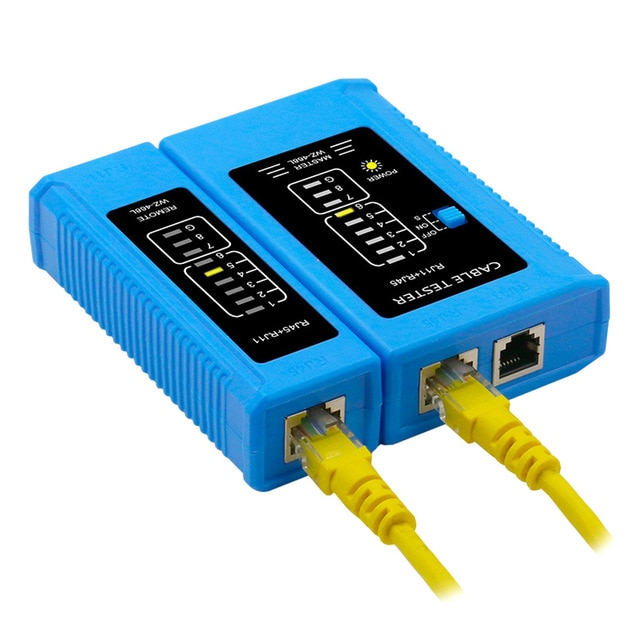
\includegraphics[scale=0.6,cframe=blue 0.5pt 3pt]{lantester.jpg} 
    \caption{LAN Cable Tester}
\end{figure}

For testing the LAN cable following steps has to  be followed:-
\begin{enumerate}
    \item Make sure both Ends are connected to their respective module(TX and RX). 
    We have to release the Wire only after hearing the clicking sound on RJ45 port.
    \item Note whether all 8 pins(led) light up , since we haven't connected any ground GND remains off.
     If the LEDs light up in order then Cable is alright and functioning and the connection is Single through.
    if not in order then there might be error during connection or the connection is Crossover.
\end{enumerate}

In one of the wire provided in the LAB  had mismatched connection so we corrected and
 tested it using  Crimping tool and LAN tester. The crimping tool provided can do multitask like can strip jacket of wire using Stripper,
 can cut wire in equal length through cutter , crimping wire to Rj45 connector using crimper and many more. 
\begin{figure}[H]
    \centering
    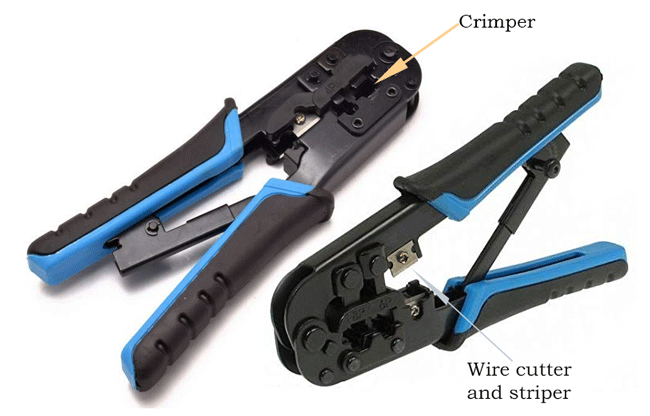
\includegraphics[scale=0.7,cframe=blue 0.5pt 3pt]{crimper-tool.png}
    \caption{Cable Crimping Tool}
\end{figure}

Following steps were followed in order to repair that faulty connection:-

\begin{enumerate}
    \item  One end of the wire was inserted to  stripping section then squeezed and rotated  which only cuts jacket and peels it off.
    \item Then the wires were straighten and arranged in order and then cut evenly, leaving only about 13mm of wire hanging.
    \item Tip of each wires were cut and copper was exposed , then inserted into the Rj45 connector such that the jacket also has space inside the connector.
    \item It was them crimped using Crimping section of Crimping tool and tested further using LAN tester.
\end{enumerate}

\pagebreak

\section{Exercises}


%%%%%%%%%%%%%%%%%%111111111111111111111111
\begin{Q}
{
    What is layered network architecture? Why layering is important?
}
\end{Q}

\begin{A}
    {
        Network Architecture can be termed as framework that direct the design and its functionality. 
        In layered network architecture the complex Network Architecture is divided into sequence of layer 
        and each assigned with particular task.Here Particular layer only interact with layer above and below it only after following protocols.
         for example:- In OSI model architecture there are 7 layers  namely :- 
        Application, Presentation, Session, Transport,Network, Data link and Physical layer.

        \begin{figure}[H]
            \centering
            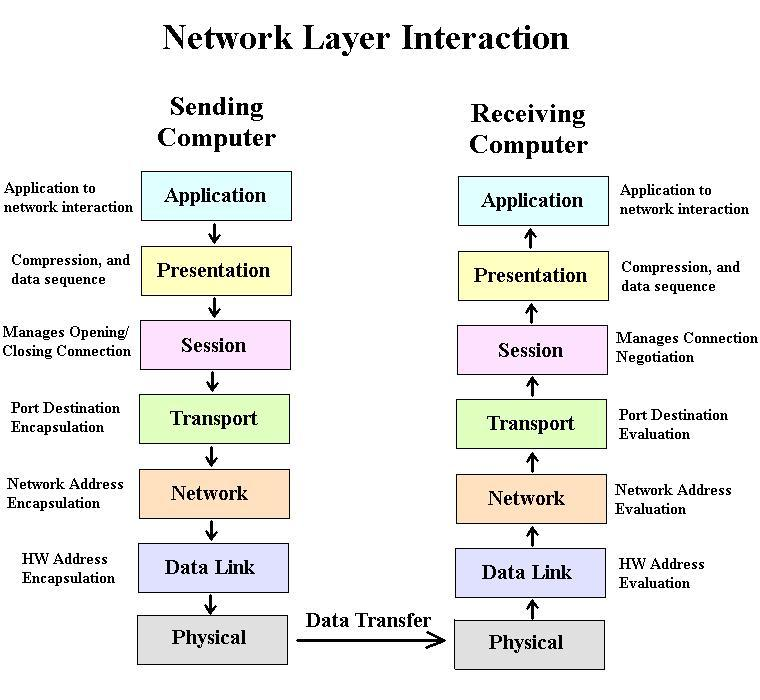
\includegraphics[scale=0.55,cframe=blue 0.5pt 3pt]{layers.jpg}
            \caption{Layered OSI Architecture}
        \end{figure}

        In Network Architecture layering is important due to following reason:-
        \begin{itemize}
            \item Using layering complex network problems can be divided in to smaller manageable tasks.
            \item It provides the Modularity Features. Each layer is independent which makes easier to implement and maintain.
            Thus providing greater  flexibility.
            \item Being the modular Design , the no. of equipment or protocol in particular layer can be altered as per the need.
            \item Being each layer independent , multiple vendors can provide support and develop the hardware .
        \end{itemize}

    }
\end{A}
%%%%%%%%%%%%%%%%%%%%%%%%%%%%%%%%%%%%%%%%%%%%%%%%%%%%%%%%%%%%%%%%%%%


%%%%%%%%%%%%%%%%%%%2222222222222222222222
\begin{Q}
    {
        What is protocol? List out ten different standard protocols having at least one in each layer of TCP/IP
        reference model.
    }
\end{Q}

\begin{A}
    {
Protocols are set of rules that need to be followed by electronics devices to format data, to transmit and receive data.
Protocols includes Data format and commands to communicate.\\

\begin{figure}[H]
    \centering
    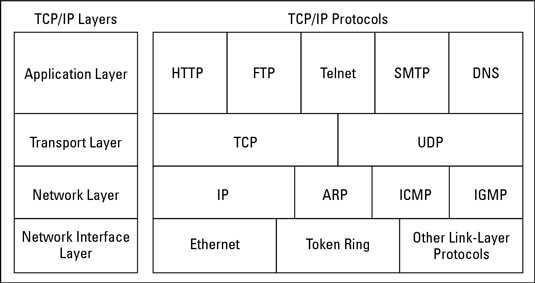
\includegraphics[scale=0.7,cframe=blue 0.5pt 3pt]{Protocols in different layers.jpg}
    \caption{Protocols in different TCP/IP layers}
\end{figure}

Different Protocols used in TCP/IP layers are:- 
\begin{itemize}
    \item \textbf{Application:} NFS, NIS+, DNS, telnet, ftp, rlogin, rsh, rcp, RIP, RDISC, SNMP,HTTP, SMTP and others
    \item \textbf{Transport:} TCP, UDP 
    \item \textbf{Internet:}IP, ARP, ICMP , IPV4,IPV6
    \item \textbf{Data Link:}PPP, IEEE 802.2 ,DSL
    \item  \textbf{Physical Network:}Ethernet (IEEE 802.3) Token Ring, RS-232, others
\end{itemize}
    }
\end{A}   
%%%%%%%%%%%%%%%%%%%%%%%%%%%%%%%%%%%%%%%%%%%%%%%%%%%%%%
\pagebreak

    %%%%%%%%%%%%%%%%%%%%%%3333333333333333333333333
\begin{Q}
    {
        List out the devices that can work up to physical, data link, network and application layer.
    }
\end{Q}

\begin{A}
    {
        The devices in each Layers are listed below:-
\begin{enumerate}
    \item \textbf{Physical}
    \begin{itemize}
        \item Hubs: Connects Segments of LAN and has multiple I/O Ports.
        \item Cables: Physical connection between devices , may include Fibers, coaxial cables and twisted pair cables.
        \item Repeaters: Regenerate or Amplify the digital or Analog signals
    \end{itemize}

    \item \textbf{Data link}
    \begin{itemize}
        \item Bridges: Provides interconnection with other network using same protocols.
        \item Modem: MOdulator/DEModulator converts Analog signal to Digital and vice-versa.
        \item  Network Interface Card (NIC): Device that connect hardware to Network.
    \end{itemize}
    
    \item \textbf{Network}
    \begin{itemize}
        \item Routers: Forwards data Packets based on IP available in Routing Tables.
    \end{itemize}
    
    \item \textbf{Application}
    \begin{itemize}
        \item Gateways: Protocols Converter which is part of two network using different protocols.
        \item Firewalls: Filters packets and prevent unauthorized access to and from Network
        \item All devices that Uses Internet, PCs ,Smartphone, Laptops etc..
    \end{itemize}
    
\end{enumerate}
    }
\end{A}
%%%%%%%%%%%%%%%%%%%%%%%%%%%%%%%%%%%%%%%%%%%%%%%%%%%%%%%%%
\pagebreak
%%%%%%%%%%%%%%4444444444444444444444444444444444444444444444444444444444444444444444444
\begin{Q}
    {
        Compare the devices (showing the similarities as well as differences):
    }
\end{Q}
%%%%%%%%%%%%%%%%%%%%%%%%%%%%%%%%%%
    \subsubsection{Repeater and Hub}
        \begin{CT}{Repeater}{Hub}
            No. of ports     & One input and One output                               & One input and many output                                       \\
    Wastage          & Doesnot cause wastage of bandwidth                     & Cause bandwidth wastage as it broadcast to all nodes available. \\
    Destination      & Doesnot check whether data reaches destination or not. & Doesnot check whether data reaches destination or not.          \\
    Collision Domain & Doesnot check for Collision Domain                     & Doesnot check for Collision Domain                              \\
    Security         & Not secure                                             & Not secure                                                      \\
        \end{CT}
%%%%%%%%%%%%%%%%%%%%%%%%%%%%%%%
    \subsubsection{Bridge and Switch}
        \begin{CT}{Bridge}{Switch}
            Layer(OSI Model)             & Data link layer                                     & Data link layer               \\
    No. of Connection & Can connect fewer LAN                               & Can connect more than Bridge  \\
    Error Checking    & Doesnot perform Error Checking                       &  Perform Error Checking       \\
    Function          & Channel Data from input port to desired output port & Divides network into segments \\
    Buffer            & May or maynot have buffer                           & Have buffer                   \\
    Speed             & Slower than switch                                  & Faster than Bridge            \\
    Table             & Use Address table                                   & Use Switch table              \\
        \end{CT}   
%%%%%%%%%%%%%%%%%%%%%%%%%%%%%%%%%%%%
    \subsubsection{Repeater and Bridge}
        \begin{CT} {Repeater}{Bridge}
            Layer(OSI Model)    & Physical layer                      & Data link layer                     \\
    NO. of ports        & One input and One output            & One input and One output            \\
    Collision Domain    & Doesnot check for Collision Domain  & Check for Collision Domain          \\
    Buffer              & Doesnot have Buffer                 & May or maynot have Buffer           \\
    Tables              & Doesnt have any Tables              & May or maynot have buffer           \\
    Security            & Not secure                          & Secure                              \\
    Cost                & Cheaper                             & Expensive                           \\
    Use                 & Extend LAN                          & Extend LAN                          \\
    Destination Address & Can't determine destination address &  Can  determine destiantion address \\
        \end{CT}





%%%%%%%%%%%%%%%%%%%%%%%%%%%%%%
    \subsubsection{Hub and Switch}
        \begin{CT}{Hub}{Switch}
            Layer(OSI Model)                  & Physical Layer                                                             & Data link layer                                                                            \\
    Table                           & Doesnot have tables for MAC address                                        & Stores MAC address in Lookup Tables                                                        \\
    Transmission Form          &  Electrical Signals and Bits                                               &  Frame Packets                                                                             \\
    Transmission Mode               & Half Duplex                                                                &  Full Duplex                                                                               \\
    Connection and Collision Domian & Can connects many  networks devices together and prone to Collision Domian & Similar to Hub but prevent collisioin domian  by directing  data to only requested devices \\
    Security                        & Not Secure                                                                 & Can be secured using VLAN.                                                                 \\
    Cost                            & Cheaper                                                                    & Expensive                                                                                  \\
         \end{CT}
%%%%%%%%%%%%%%%%%%%%%%%%%%%%%%%%%%%%%%%%%%%
    \subsubsection{Switch and Router}
        \begin{CT}{Switch}{Router}
            Layers(OSI Model)   & Data link layer                          & Network layer                            \\
            Tables              & Switch table to store MAC                & Routing table to store IP address        \\
            NAT                 & Cannot perform NAT                       & Can perform NAT                          \\
            Network Type        & Operate on Wired Network Only            & Operate on Wireless and wired network    \\
            Destiantion Address & Knows destination address of data packet & Knows destination address of data packet \\
            Operation Area      & LAN                                      & Used in all LAN, MAN ,WAN                \\
            Transmission Mode   & Full duplex mode transmission            & Full duplex mode transmission            \\
        \end{CT}

%%%%%%%%%%%%%%%%%%%%%%%%%%%%%%%%%%%%%%%%%%%%%%%
    \subsubsection{Router and Gateway}
        \begin{CT}{Router}{Gateway}
            Layers(OSI Model) & Network                                                          & All Layers                                                               \\
            Working           & Receive ,Analyze and Forward the data                            & Communication Among Networks using different protocols                   \\
            Function          & Route Traffice between the Network                               & Translate protocol                                                       \\
            Dynamic Routing   & Supported                                                        & Not Supported                                                            \\
            Hosted on         & Dedicated Application (Physical Hardware)                        & Can be on Dedicated Application , Physical server or Virtual Application \\
            Features          & DHCP.NAT.Static Routing,Wireless,IPV6,Mac address filtering etc. & Voip to PSTn or Network Access Control                                   \\
        \end{CT}
%%%%%%%%%%%%%%%%%%%%%%%%%%%%%%%%%%%%%%%%%%%%%%%
\pagebreak
%%%%%%%%%%%%%%%%%%%%%%5555555555555555555555555
\begin{Q}
    {
        Why logical addressing is required in network communication? Explain briefly.
    }
\end{Q}

\begin{A}
    {
In networking there are two types of addressing  Logical and Physical.
Physical addressing useS manufacture assigned MAC address for identity where as 
Logical addressing uses virtual assigned  IP address.\\

The main reason for using Logical address instead of MAC is to forward the traffic effectively across the globe.
Manufacture assign consecutive product, the consecutive MAC address but those product may end on the opposite side of the globe.
So, when Mac is used the data packet has to travel back and forth around the globe until it reaches the destination.
In order to solve this issue Logical addressing is in use. It is assigned to a device as per their Location(ISP). so, the data packet 
intended for that device can first travel to ISP then to the device easily.

    }
\end{A}
%%%%%%%%%%%%%%%%%%%%%%%%%%%%%%%%%%%%%%%%%%%%%%%

%%%%%%%%%%%%%%%%%%%%%%%666666666666666666666666666
\begin{Q}
    {
        Where do you need straight-through and cross-over cable? Explain briefly.
    }
\end{Q}

\begin{A}
    {
        \begin{figure}[H]
            \centering
            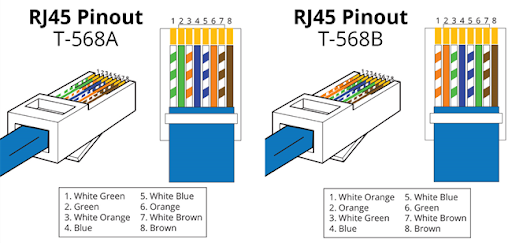
\includegraphics[scale=0.9,cframe=blue 0.5pt 3pt]{T568ab.png}
            \caption{T-568A and T-568B Color coding}
        \end{figure}
        There are basically two wiring standard in Networking T-568A and T-568B flowing different color code.
        There are two wiring technique Straight through and Crossover Cable. 

        \begin{figure}[H]
            \centering
            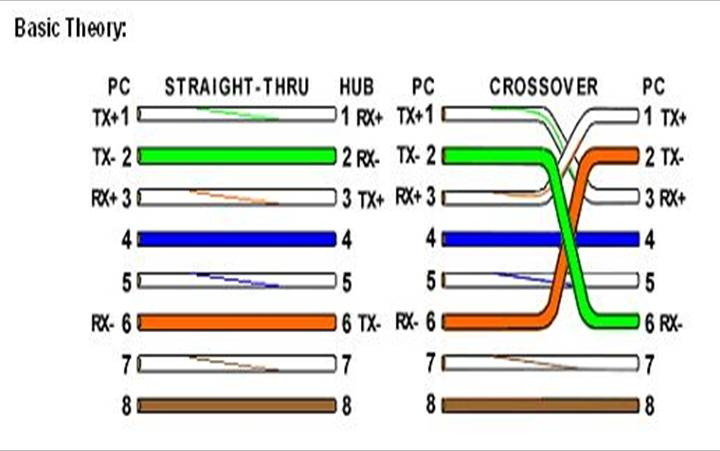
\includegraphics[scale=0.5,cframe=blue 0.5pt 3pt]{straight cross.jpg}
            \caption{Difference in Straight through and Cross over}
        \end{figure}

        In straight through both ends of the wire follows the same wiring standard whereas 
         in Crossover  wiring standard of one ends doesn't match with others. 
         To put in other words if pin 1 and 2 of one ends is connected to 3 and 6 of other then such connection Crossover.
         
         \begin{figure}[H]
            \centering
            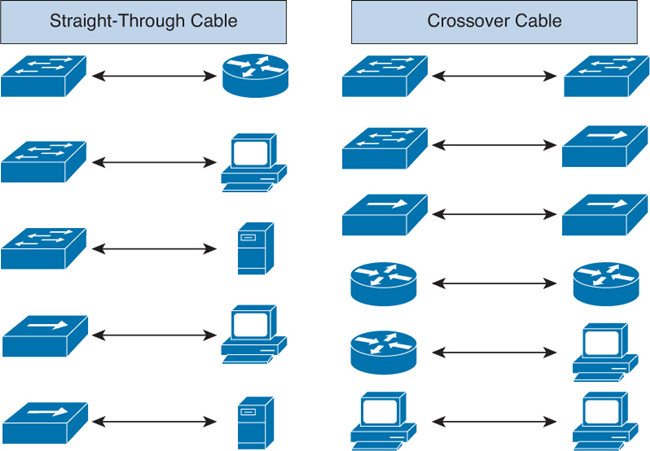
\includegraphics[scale=0.6,cframe=blue 0.5pt 3pt]{Choose-Straight-Through-or-Crossover-Cable.jpg}
            \caption{Application of Straight through and  Cross over}
        \end{figure}

        \begin{table}[H]
            \begin{tabular}{|l|l|l|l|l|}
            \hline
            \textbf{DEVICES}                         & \textbf{Hub} & \textbf{Switch} & \textbf{Router} & \textbf{Workstation} \\ \hline
            \textbf{Hub}         & Crossover               & Crossover                  & Striaght                   & Striaght                        \\ \hline
            \textbf{Switch}      & Crossover               & Crossover                  & Striaght                   & Striaght                        \\ \hline
            \textbf{Router}      & Striaght                & Striaght                   & Crossover                  & Crossover                       \\ \hline
            \textbf{Workstation} & Striaght                & Striaght                   & Crossover                  & Crossover                       \\ \hline
            \end{tabular}
        \end{table}
}
\end{A}
%%%%%%%%%%%%%%%%%%%%%%%%%%%%%%%%%%%%%%%%%%%%%%%





\section{Conclusion}
This lab started with introduction to Computer network and devices involved in different layers,
like switch ,hub ,Routers and then we move to different cables and connectors and all the way to cable tester and  Rj45 cable with Crimping tool.
In this lab we also got familiar with  Straight through  and crossover cable connection and their practical uses.

\end{document}

